\documentclass[11pt,a4paper]{book}
\usepackage{titlesec}
\usepackage{setspace}
\usepackage{graphicx}
\usepackage{wrapfig}
\usepackage{color,soul}
\usepackage[customcolors,shade]{hf-tikz}
\usepackage{amsmath}
\usepackage{amssymb}
\usepackage{graphicx}
\usepackage{subfig}
\usepackage{sidecap}
\graphicspath{{/Users/giuliodilernia/Documents/Laboratory-Notes/Teoria_Lab2/images/}}

\renewcommand{\baselinestretch}{1.3} 

\titleformat{\chapter}[display]
 {\bfseries\Large}
  {\filright\MakeUppercase{\chaptertitlename} \Huge\thechapter}
  {1ex}
  {\titlerule\vspace{1ex}\filleft}
  [\vspace{1ex}\titlerule]

\begin{document}
\setcounter{chapter}{3}
\chapter{Stime di Parametri}


\section{La statistica}
La statistica studia il problema di inferire da un campione i parametri e/o i modelli che descrivono la popolazione dalla quale il campione \`{e} stato estratto. In particolare possiamo dividerla in due categorie:

\begin{itemize}
	\item Stima dei parametri, misura di una quantit\`{a} fisica;
	\item Test d'ipotesi, ovvero la prova della validit\`{a} di un modello.
\end{itemize}

Una funzione dipendente da N misure di un campione $f(x_1,...,x_n)$ si chiama \textbf{statistica}, essa \`{e} una \textbf{variabile aleatoria}. Quindi segue una sua distribuzione di probabilit\`{a} $pdf_f$ derivabile dalla joint-pdf dei campionamenti e dalla forma della funzione f.

\noindent Complessivamente si hanno 3 pdf:
\begin{itemize}
	\item la $pdf_x$(x,$\theta$) delle singole misure campionate; 
	\item la $pdf_{set}$($x_1,...,x_n,\theta)$ dei campionamenti (che \`{e} multidimensionale);
	\item la $pdf_f$ della statistica dei campionamenti (dipende dalla forma funzionale di f).
\end{itemize}


\section{Stimatori}

Sia data una p.d.f. (probability distribution function), $f(x,\theta)$ di una variabile x aleatoria  continua e dipendente da un parametro $\theta$, di cui non conosciamo il vero valore $\theta_{true}$.
\newline
Se si possiede un insieme $\{x_i\}_i^N$ di N misure della variabile x, possiamo chiederci se sia possibile determinare una stima del parametro $\theta_{true}$ in funzione di tali misure, $\hat{\theta} = \hat{\theta}(x_1,....,x_N)$, le funzioni di questo tipo prendono il nome di \textbf{stimatori}. Uno stimatore \`{e} una statistica opportunamente scelta. Con \textbf{stima} s'intende il valore assunto $\hat{\theta}^*$ dallo stimatore per uno specifico campione. 


\begin{figure}[ht]
\vspace{0.6in}

\includegraphics[scale = 1.3]{N_measure}	
\centering
\vspace{0.3in}
\caption{N misure}
\end{figure}

\noindent Poich\`{e} lo stimatore $\hat{\theta}$ \`{e} dipende da variabili aleatorie \`{e} anch'esso  una variabile aleatoria e dunque si pu\`{o} parlare di valore medio $E[\hat{\theta}]$ e varianza $V[\hat{\theta}]$ di una particolare stima, oltre ad avere una sua pdf$(\hat{\theta})$.

\begin{equation}
	\hat{\theta} \pm \sigma_{\theta}
\end{equation} 

Di conseguenza un insieme di misure restituir\`{a} un solo valore appartenente ad una popolazione ottenuta da campione fatto di misure della variabile aleatoria presa in considerazione.

\section{Propriet\`{a} degli stimatori}

Consideriamo un campione di N misure $\{x_i\}_i^N$ vengono definite IID (Independent Identically Distributed) quando sono:
\begin{itemize}
	\item \textbf{indipendenti:} l'esito di una misura non \`{e} influenzato dalle misure precedenti;
	\item \textbf{identiche:} Delle misure vengono definite identiche quando tutte quante seguono la stessa distribuzione di probabilit\`{a}
\end{itemize}
Nella statistica alle stime si possono associare diverse caratteristiche :

\begin{enumerate}
	\item \textbf{Consistenza:} una stima si dice consistente quando all'aumentare del numero di misure (convergenza probabilistica) si converge al valore vero del parametro. Ossia quando:
	\begin{equation}
		\lim_{N \rightarrow \infty} \hat{\theta}(x_1,.....,x_N) = \theta_{true} 
	\end{equation}
	 
\begin{figure}[ht]
\vspace{0.6in}
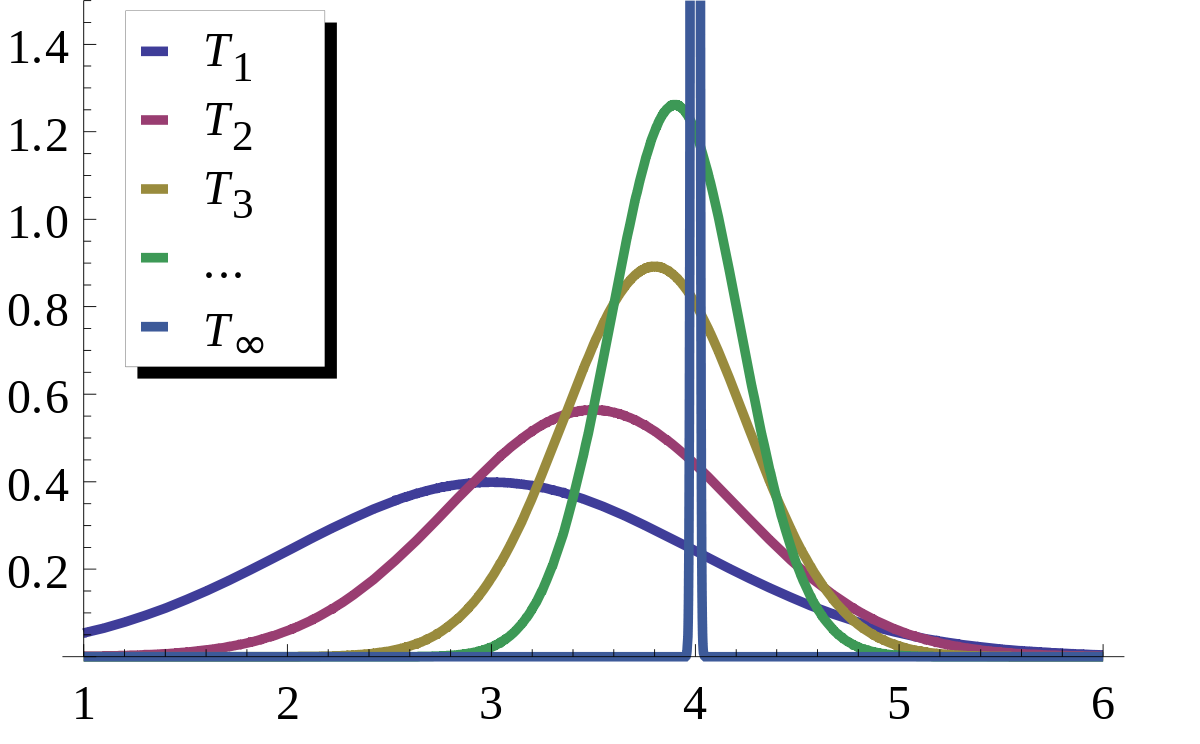
\includegraphics[scale = 0.2]{ConsistentEstimator}	
\centering
\vspace{0.3in}
\caption{Propriet\`{a} di consistenza di uno stimatore}
\end{figure}
	
	\item \textbf{Biased}: 
	\begin{enumerate}
	\item una stima si dice unbiased o imparziale, se mediamente coincide con il valore vero del parametro, ovvero 
	\begin{equation}
		b_{n}(\hat{\theta}) = E(\hat{\theta}_n - \theta_{true}) = E(\hat{\theta}_n) - E(\theta_{true}) = 0 
		\iff E(\hat{\theta_n}) = \theta_{true} 
	\end{equation}
	
	\item Una stima si dice asintoticamente unibiased se $b_n(\hat{\theta}) \rightarrow 0$ per $n \rightarrow \infty $.\newline
	\end{enumerate}
	Si osserva che $b_n{}(\hat{\theta})$ \`{e} uno stimatore lineare, dunque se $\hat{\theta}$ \`{e} stimatore di $\theta_{true}$ questo non vuol dire che $\hat{\theta}^2$ \`{e} stimatore di $\theta_{true}^2$.
	
	 
\begin{figure}[!ht]
\vspace{0.3in}
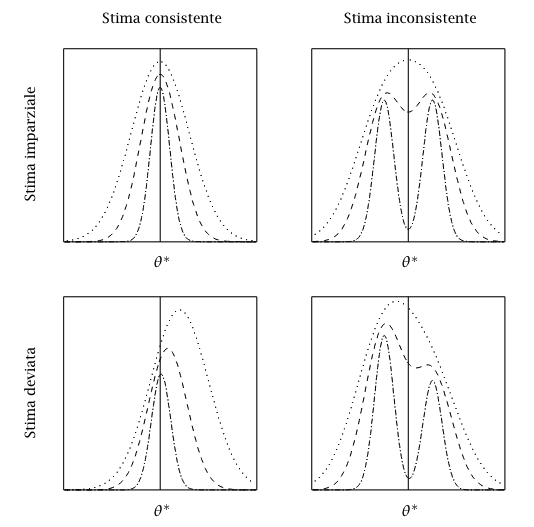
\includegraphics[scale = 0.5]{Stimatore}	
\centering
\vspace{0.3in}
\caption{Consistenza e Bias di uno stimatore}
\end{figure}
	
\item \textbf{Efficienza}: si dice che una stima \`{e} pi\`{u} efficiente di un'altra se la sua varianza \`{e} inferiore, quindi se mediamente essa \`{e} pi\`{u} vicina al valore centrale $E(\hat{\theta})$, che coincide con $\theta_{true}$ se la stima \`{e} anche imparziale (ubiased). 

\item \textbf{Varianza:} desideriamo che ripetendo i campionamenti le stime ottenute siano tutte vicine tra loro, ovvero la varianza della $pdf(\hat{\theta})$ sia il pi\`{u} piccola possibile.
\end{enumerate}

\subsection{Precisione e Accuratezza}

 Per uno stesso parametro si possono in generale definire tanti stimatori diversi tra loro, ma non tutti hanno le propriet\`{a} desiderate. Da notare che non \`{e} detto che esista (o sia possibile trovare) uno stimatore che soddisfi contemporaneamente tutte le propriet\`{a} richieste.
\subsubsection{Esempio} 

La media delle misure \`{e} uno stimatore non distorto. \newline

Dim.
\newline
Definito come stimatore la media aritmetica delle misure di un campione IID:
\begin{equation*}
		 \hat{\mu} = \frac{1}{N}\sum{x_{i}} 
\end{equation*}
si ha che il valore di aspettazione dello stimatore \`{e}:
\begin{equation*}
	  E(\hat{\mu})= E(\frac{1}{N}\sum x_{i})= \frac{1}{N}\sum E(x_{i})= \frac{1}{N} \cdot N \cdot \mu_{t} = \mu_{t} 
\end{equation*}
quindi la media aritmetica \`{e} uno stimatore \textbf{non distorto} poich\`{e}:
\begin{equation*}
	 b_n(\hat{\mu}) = E(\hat{\mu}) - \mu_{t} = \mu_{t} - \mu_{t} = 0  
\end{equation*}

\noindent Se la pdf(x) delle misure soddisfa le ipotesi del TCL, la pdf($\hat{\mu})$ per $N \rightarrow \infty$ tende a una \textbf{gaussiana} con media $\mu$ e varianza $\frac{\sigma^2}{N}$ si ha che $\hat{\mu}$ \`{e} uno stimatore \textbf{consistente}. Poich\`{e} $V[\hat{\mu}] = \frac{\sigma^2}{N}$ al crescere del numero di campionamenti la varianza si riduce e dunque le stime ottenute con diversi set di dati sono tutte vicine tra loro.


\subsection{Incertezze sulle stime}

\noindent Uno stimatore come ogni altra variabile aleatoria \`{e} soggetto a due tipi d'incertezze:

\begin{enumerate}
	\item \textbf{Incertezza sistematica:} nel caso di misure biased esiste una differenza sistematica fra la misura sperimentale ottenuta e il valor vero, ed \`{e} uguale per tutte le misure e non \`{e} possibile determinarlo essendo una propriet\`{a} intrinseca.
	\item \textbf{Incertezza statistica:} \`{e} associata alla precisione, e la si pu\`{o} ridurre aumentando il numero di misure o cambiando l'apparato sperimentale.
\end{enumerate}
\begin{equation}
		MSE =E[(\hat{\theta} -\theta_t)^2] =Var(\hat{\theta)} \: + \; b_{n}^2(\hat{\theta}) 
\end{equation}

Definisce l'errore quadratico medio e tiene conto sia dell'errore statistico misurato dalla varianza che dell'errore sistematico misurato dal bias.
\subsection{La Varianza come stimatore}

Consideriamo di avere un insieme di N misure, $\{x_{i}\}_{i}^N$ di cui conosciamo il valore medio $\mu$ della popolazione e di volerne determinare la varianza, poich\`{e} essa dipende dalle misure del campione \`{e} una variabile aleatoria a sua volta e dunque da un campione definiamo una stima del valore reale del parametro $\sigma_{t}$. Di conseguenza possiamo domandarci le propriet\`{a} che tale stimatore possiede.
	\newline
Definiamo lo stimatore varianza come:		
\begin{equation*}
		 \hat{\sigma}_{\mu}^2(x) = \frac{1}{N} \sum{(x_{i}-\mu})^2 \quad \text{oppure} \quad   \hat{\sigma}^2(x) = E(x^2) - E(x)^2
\end{equation*}

\noindent Verifichiamo che la varianza sia uno stimatore non distorto ovvero che:

\begin{equation*}
		E(\hat{\sigma}^2) = \sigma_{t}	
\end{equation*}

\noindent Per farlo sfruttiamo la porpriet\`{a} di linearit\`{a} del valore atteso.
\newline
Dim.
\begin{align*}	
		& E(\hat{\sigma}_{\mu}^2) = E(\frac{1}{N} \sum{(x_{i}-\mu})^2) = \frac{1}{N}\sum(E(x_i^2) - 2\mu E(x_i)+\mu^2) =
		\\
		\\
		 & = \frac{1}{N}\sum(E(x_i^2) - 2\mu E(x_i)+\mu^2) = \frac{1}{N}\sum(E(x_i^2) -\mu^2) = \frac{1}{N} \cdot N \cdot \sigma_t = \sigma_t
\end{align*}
\newline
\noindent Dunque la varianza \`{e} uno stimatore non distorto nel caso in cui si conosca il valore medio della popolazione. Raramente si conosce $\mu$ della popolazione, dunque consideriamo come stimatore la varianza per un campione di N misure IID.
\begin{equation*}
	\hat{\sigma}_{\overline{x}}^2 = \dfrac{1}{N}\sum_{i=1}^N(x_i - \overline{x})^2	
\end{equation*}
\newline
\noindent Sappiamo che la varianza determina la dispersione di un campione di misure attorno alla sua media. Ipotizziamo di conoscere il valore medio del campione $\overline{x}$, per costruzione risulta essere il valore pi\`{u} vicino alle misure dell'insieme. La media della popolazione $\mu$ non necessariamente coincide con $\overline{x}$ del campione, e dunque pu\`{o} non essere il valore attorno al quale si distribuiscono le misure del campione; infatti nel caso in cui non lo sia al crescere del numero di misure questo pu\`{o} diventare il valore pi\`{u} distante rispetto a $\overline{x}$ stimato dal campione iniziale. Le distanze quadratiche da  $\overline{x}$ saranno quindi una sottostima di $\mu$ e quindi anche $\hat{\sigma}$ sar\`{a} uno sottostima di $\sigma_t$.  
 \begin{align*}
		&E[\hat{\sigma}_{\overline{x}}^2] = \frac{1}{N} \sum{E(x_{i}^2}) - E([\frac{1}{N}\sum{x}_{i}]^2) = \sigma_{t}(x)^2 + \mu^2 - \frac{1}{N^2}[\sigma_{t}^2(\sum{x_{i}}) + E(\sum{x_{i}})^2] = 
		\\
		\\
		&= \sigma_{t}(x)^2 + \mu^2 - \frac{1}{N^2}[N\sigma_{t}^2(x) + N^2 \mu^2] = \sigma_{t}^2(x) \Big[\frac{N-1}{N} \Big ] 
\end{align*}
 
\noindent Di conseguenza la varianza di un campione $\hat{\sigma}_{\overline{x}}$ \`{e} uno stimatore distorto, infatti:
\begin{equation*}
	b_n[\hat{\sigma}_{\overline{x}}^2] = E[\hat{\sigma}_{\overline{x}}^2] - \sigma_{t}^2 = \sigma_{t}^2(x) \Big[\frac{N-1}{N} \Big ] - \sigma_{t}^2 
\end{equation*}
ma \textbf{asintoticamente non distorto} poich\`{e} per $N \rightarrow \infty $ si ha $b_n[\hat{\sigma}_{\overline{x}}^2] \rightarrow 0$.
\newline

\noindent Notare che quest'ultima definizione \`{e} quella operativa per verficiare che la varianza sia uno stimatore non ubiased in quanto difficilmente si conosce il valore medio $\mu$ della popolazione. 

\subsection{Correzione di Bessel}

Si pu\`{o} definire un terzo stimatore, che introduca una correzione a $\hat{\sigma}_{\overline{x}}^2$ tale da cancellare il bias. La correzione del bias \`{e} applicabile tutte le colte in cui il bias \`{e} precisamente noto. Il nuovo stimatore della varianza sar\`{a} dato da:

\begin{equation}
	s^2 \equiv \dfrac{1}{N-1} \sum_{i=1}^N (x_i - \overline{x})^2
\end{equation}
\newline
e prende il nome di \textbf{correzione di Bessel}.
\newline
Lo stimatore \`{e} unbiased $E[s^2] = \sigma_t^2$, ma la varianza di tale stimare non pu\`{o} essere determinata per il caso generale

\begin{equation*}
	V[s^2] = V[\dfrac{1}{N-1} \sum_{i=1}^N (x_i - \overline{x})^2] = \dfrac{1}{(N-1)^2} \sum_{i=1}^N V[(x_i - \overline{x})^2]
\end{equation*}
\newline
ma \`{e} possibile farlo solo nel caso in cui il campione di misura segue una pdf(x)\textbf{ Gaussiana}.
\begin{figure}[!ht]
\vspace{0.1in}
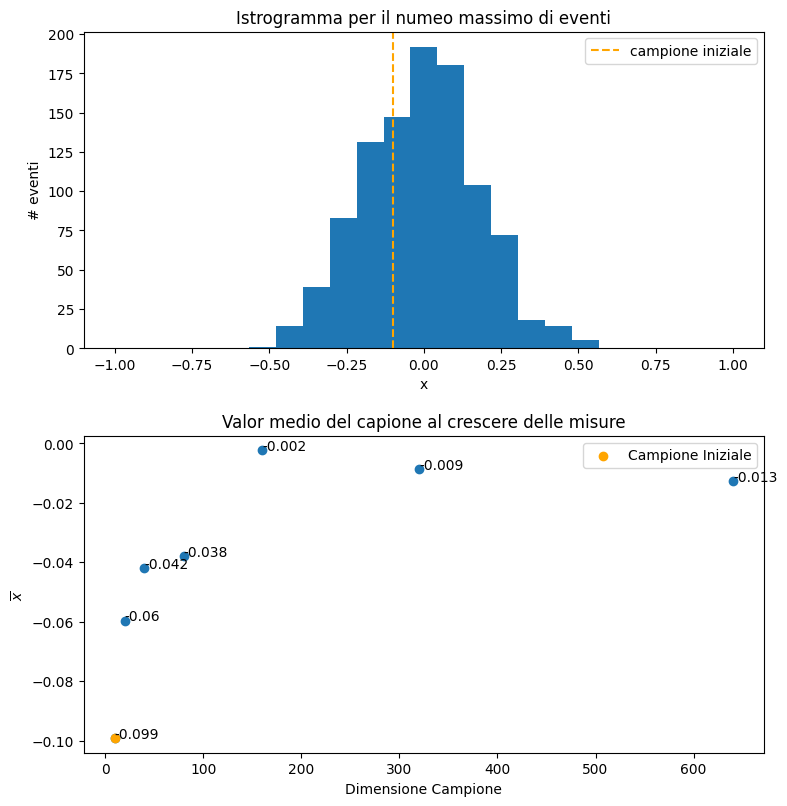
\includegraphics[scale = 0.5]{VarianceBiased}	
\centering
\vspace{0.3in}
\caption{Misure casuali che seguono una pdf di Gauss tra -1 e 1 in cui $\overline{x}$ del campione iniziale non coincide con il valore medio $\mu = 0$ della popolazione. Dunque $\overline{x}$ non \`{e} pi\`{u} il centro del campione al crescere delle misure. }
\end{figure}

\noindent Se riscriviamo lo stimatore $s^2$ nel seguente modo:

\begin{equation*}
s^2 \equiv \dfrac{1}{N-1} \sum_{i=1}^N (x_i - \overline{x})^2 = \dfrac{\sigma_t^2}{N-1} \textcolor{red}{\sum_{i=1}^N \dfrac{(x_i - \overline{x})^2}{\sigma_t^2}}
\end{equation*}
possiamo introdurre una variabile aleatoria ausiliaria definita come $\textcolor{red}{\chi^2}$ e riscrivere $s^2$ come:

\begin{equation*}
	s^2 \equiv \dfrac{\sigma_t^2}{N-1}\textcolor{red}{\chi^2}
\end{equation*}
\newline
di conseguenza $V[s^2]$ \`{e} legata alla $V[\textcolor{red}{\chi^2}]$. Nell'ipotesi in cui le misure raccolte seguano una distribuzione di probabilit\`{a} Gaussiana la variabile $\chi^2$ segue la distribuzione del chi-quadro. Tale pdf \`{e} descritta da un solo parametro definito gradi di libert\`{a} e nel nostro caso tale parametro vale N-1. 
\newline
Di conseguenza con questa nuova distribuzione possiamo dimostrare che $s^2$ \`{e} uno stimatore non distorto.\newline

Dim.

\begin{equation*}
	E[s^2] = E \Big[\dfrac{\sigma_t^2}{N-1}\textcolor{red}{\chi^2} \Big] = \dfrac{\sigma_t^2}{N-1}E[\textcolor{red}{\chi^2}] = \dfrac{\sigma_t^2}{N-1}(N-1) = \sigma_t^2
\end{equation*}
\newline
La sua varianza \`{e} data da:

\begin{equation*}
	V[s^2] = V \Big [ \dfrac{\sigma_t^4}{(N-1)^2}\textcolor{red}{\chi^2} \Big] = \dfrac{\sigma_t^4}{(N-1)^2}V[\textcolor{red}{\chi^2}] = \dfrac{2\sigma_t^4}{(N-1)^2} 
	\end{equation*}

\section{Intervallo di confidenza}

Si \`{e} costruito uno stimatore $\hat{\theta}$ per un parametro $\theta$ che \`{e} una variabile aleatoria di conseguenza esiste una distribuzione pdf($\hat{\theta}$) che \`{e} caratterizzata da una media E[$\hat{\theta}$] e una varianza V[$\hat{\theta}$]. La \textbf{stima} \`{e} il valore che lo stimatore assume in corrispondenza di un campione di dati e lo definiamo $\hat{\theta}^*$.\newline

\noindent L'\textbf{intervallo di confidenza} \`{e} solitamente indicato come:
\begin{equation}
	\hat{\theta}^* \pm \sigma \quad \text{oppure} \quad \hat{\theta}^* \; \begin{matrix}
		+\sigma_1 \\ - \sigma_1
	\end{matrix}
\end{equation}
la seconda notazione viene usata quando l'intervallo \`{e} asimmetrico. \newline
\begin{wrapfigure}{r}{0.5 \textwidth}

\vspace{-10pt}
\centering
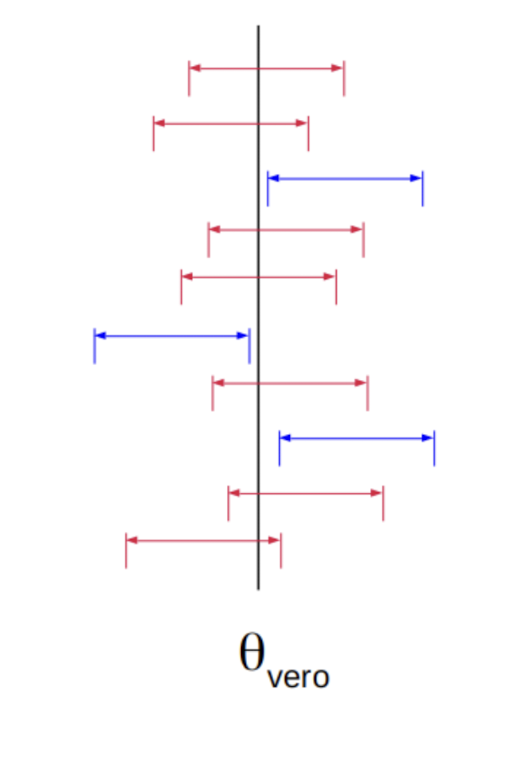
\includegraphics[width = 0.4 \textwidth]{interval}	

\end{wrapfigure}
In generale il risultato della stima \`{e} un intervallo [a,b], poich\`{e} \`{e} una variabile aleatoria si ha che gli estremanti sono variabili aleatorie e dunque per diversi campioni si hanno diversi intervalli di confidenza. A ciascun intervallo viene associata una probabilit\`{a} (\textbf{livello di confidenza}) che misura quanto \`{e} buona la stima del valore vero.

\begin{equation*}
	P(\theta_t \in [a,b])
\end{equation*}
dove essa rappresenta la frazione delle volte in cui ripetendo l'esperimento, la stima restituisce un intervallo che contiene il valore vero.\newline

In generale si vuole trovare un metodo che individui un intervallo [a,b] tale per cui la probabilit\`{a} che $\theta_t \in [a,b]$ sia pari a un certo valore $\beta$ detto \textbf{livello di confidenza}. Un intervallo di confidenza cos\`{i} definito prende il nome di \textbf{intervallo di condifenza di Neyman}. Un intervallo particolare \`{e} quello dato da $[\hat{\theta}^* - \sigma, \hat{\theta}^* + \sigma]$ e si definisce \textbf{intervallo centrale}.



\end{document}